\documentclass[11pt]{article}

\usepackage[a4paper,margin=1in]{geometry}
\usepackage{amsmath,amssymb,bm}
\usepackage{graphicx}
\usepackage{float}
\usepackage{booktabs}
\usepackage{microtype}
\usepackage{siunitx}
\usepackage{hyperref}
\usepackage{tcolorbox}

\title{Quadruple-Tank (Coupled Tanks) Modeling\\State Space and Transfer Function Forms}
\author{Adha Imam Cahyadi, Dr.Eng\\Assoc.\ Professor in Dynamic Control Systems\\Department of Electrical Engineering, Universitas Gadjah Mada}
\date{\today}

\begin{document}
\maketitle

\section{Purpose}
\begin{tcolorbox}[colback=blue!5!white, colframe=blue!75!black, title=Purpose]
These notes provide a compact modeling workflow for the quadruple-tank (coupled tanks) process:
\begin{itemize}
  \item nonlinear physical model (mass balance + Torricelli outflow),
  \item linearization about an operating point,
  \item state-space model \(\dot{\bm{x}} = A\bm{x} + B\bm{u}, \ \bm{y} = C\bm{x} + D\bm{u}\),
  \item transfer-function matrix \(G(s)\) relating inputs to outputs in the frequency domain.
\end{itemize}
\end{tcolorbox}

\paragraph{Controller restriction (course rule).}
In this project, students design controllers \emph{in the frequency domain} using either:
\begin{itemize}
  \item lead--lag compensators, or
  \item PID controllers (interpreted as a frequency-domain compensator \(C(s)\)).
\end{itemize}
Time simulation is used only to \emph{validate} frequency-domain designs (e.g., check actuator limits and nonlinear effects).

\begin{figure}[H]
  \centering
  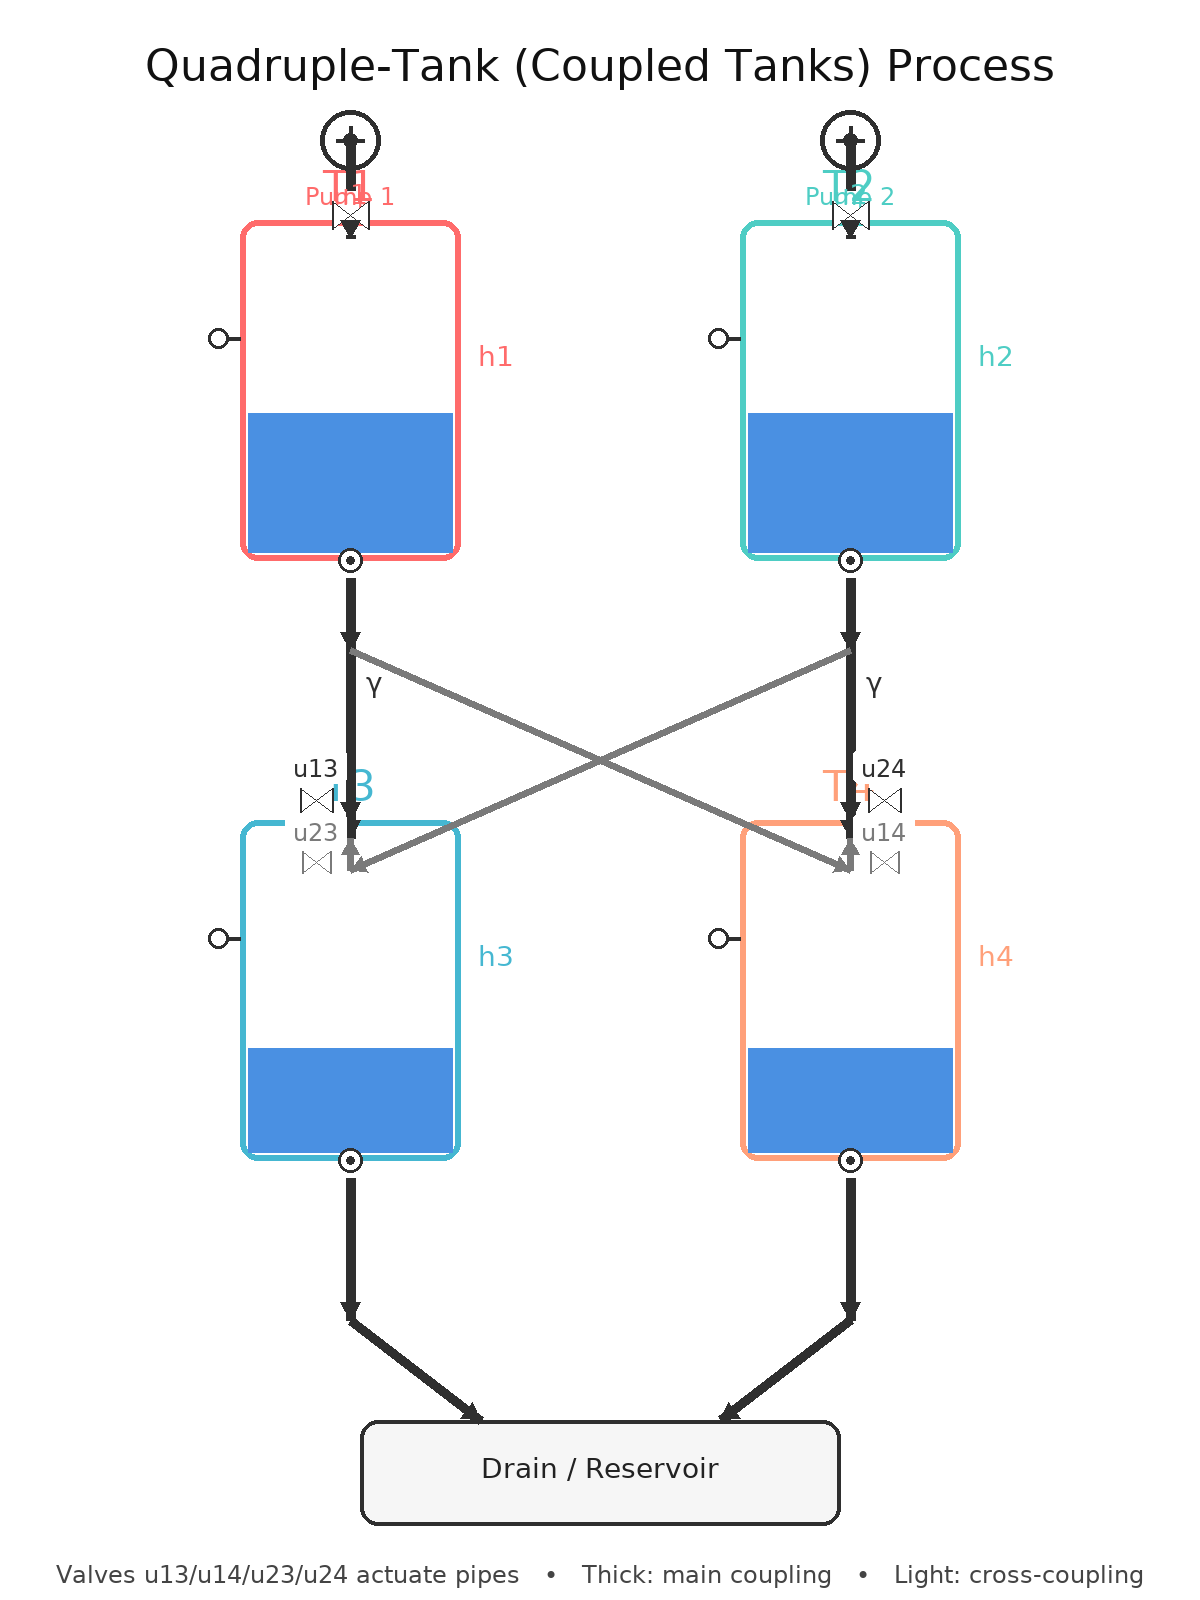
\includegraphics[width=0.62\textwidth]{system_diagram_realistic.png}
  \caption{Quadruple-tank laboratory process schematic (two pumps, four tanks, cross-coupled upper-to-lower flows, and a drain/reservoir).}
  \label{fig:schematic}
\end{figure}

\section{Variables, inputs, and parameters}
\subsection*{States and signals}
\begin{align*}
\bm{x} &= \begin{bmatrix} h_1 & h_2 & h_3 & h_4 \end{bmatrix}^\top
&&\text{tank levels (heights)}\\
\bm{u} &= \begin{bmatrix} u_1 & u_2 \end{bmatrix}^\top
&&\text{manipulated inputs (default: two pump inflows)}\\
\bm{y} &= \begin{bmatrix} y_1 & y_2 \end{bmatrix}^\top
&&\text{measured outputs (typically }y_1=h_1,\ y_2=h_2\text{)}
\end{align*}

\subsection*{Physical parameters (typical)}
\begin{itemize}
  \item \(A_i\): cross-sectional area of tank \(i\) \([\si{cm^2}]\).
  \item \(a_i\): outlet (orifice) area of tank \(i\) \([\si{cm^2}]\).
  \item \(g\): gravity \([\si{cm/s^2}]\) (often \(g \approx 981\ \si{cm/s^2}\)).
  \item \(C_d\): discharge coefficient (dimensionless).
  \item \(c_{13},c_{14},c_{23},c_{24}\): coupling coefficients mapping upper-tank outflows into lower-tank inflows (dimensionless).
  \item \(k_1, k_2\): pump gains converting command to inflow \([\si{cm^3/s}]\) (often \(k_1=k_2=1\) if the input is already flow).
\end{itemize}

\paragraph{Note.}
Different lab rigs/papers use different interconnection conventions. The equations below match this repository's implementation, where tank 3 and tank 4 inflows are linear combinations of upper-tank outflows using coefficients \(c_{13},c_{14},c_{23},c_{24}\). See \path{quadruple_tanks/models/quadruple_system.py}.


\section{Nonlinear model (mass balance + Torricelli outflow)}
\subsection{Outflow (Torricelli)}
For each tank \(i\),
\begin{align}
q_i(h_i) &= C_d\, a_i \sqrt{2 g h_i}
\qquad (h_i \ge 0)
\label{eq:torricelli}
\end{align}
where \(q_i\) is the volumetric outflow \([\si{cm^3/s}]\).

\subsection{Inflow structure (coupling)}
\begin{align*}
q_{3,\text{in}} &= c_{13}\, q_1(h_1) + c_{23}\, q_2(h_2)\\
q_{4,\text{in}} &= c_{14}\, q_1(h_1) + c_{24}\, q_2(h_2)
\end{align*}
Upper tanks receive pump inflows:
\begin{align*}
q_{1,\text{in}} &= k_1 u_1,\qquad
q_{2,\text{in}} = k_2 u_2
\end{align*}

\subsection{State equations}
Using \(\dot{h}_i = (q_{i,\text{in}} - q_i)/A_i\), the nonlinear dynamics are
\begin{align}
\dot{h}_1 &= \frac{k_1 u_1 - q_1(h_1)}{A_1}
\label{eq:h1_nl}\\
\dot{h}_2 &= \frac{k_2 u_2 - q_2(h_2)}{A_2}
\label{eq:h2_nl}\\
\dot{h}_3 &= \frac{c_{13}\, q_1(h_1) + c_{23}\, q_2(h_2) - q_3(h_3)}{A_3}
\label{eq:h3_nl}\\
\dot{h}_4 &= \frac{c_{14}\, q_1(h_1) + c_{24}\, q_2(h_2) - q_4(h_4)}{A_4}
\label{eq:h4_nl}
\end{align}

\section{Operating point and linearization}
\subsection{Equilibrium (steady state)}
Choose a steady operating point \((\bm{x}_0,\bm{u}_0)\) such that \(\dot{\bm{x}}=\bm{0}\).
From \eqref{eq:h1_nl}--\eqref{eq:h2_nl}:
\begin{align}
k_1 u_{1,0} &= q_1(h_{1,0}), \qquad
k_2 u_{2,0} = q_2(h_{2,0})
\label{eq:upper_eq}
\end{align}
and from \eqref{eq:h3_nl}--\eqref{eq:h4_nl}:
\begin{align}
q_3(h_{3,0}) &= c_{13}\, q_1(h_{1,0}) + c_{23}\, q_2(h_{2,0}) \\
q_4(h_{4,0}) &= c_{14}\, q_1(h_{1,0}) + c_{24}\, q_2(h_{2,0})
\end{align}

\subsection{Small-signal variables}
Define perturbations around the operating point:
\[
\tilde{\bm{x}} = \bm{x} - \bm{x}_0,\qquad
\tilde{\bm{u}} = \bm{u} - \bm{u}_0,\qquad
\tilde{\bm{y}} = \bm{y} - \bm{y}_0
\]
The linearized model is
\begin{align}
\dot{\tilde{\bm{x}}} &= A\,\tilde{\bm{x}} + B\,\tilde{\bm{u}}
\label{eq:ss_lin}\\
\tilde{\bm{y}} &= C\,\tilde{\bm{x}} + D\,\tilde{\bm{u}}
\label{eq:out_lin}
\end{align}

\subsection{Derivative of the outflow}
From \eqref{eq:torricelli},
\begin{align}
\frac{d q_i}{d h_i}\bigg|_{h_{i,0}}
&= C_d a_i \frac{g}{\sqrt{2 g h_{i,0}}}
= \frac{C_d a_i \sqrt{2g}}{2\sqrt{h_{i,0}}}
\triangleq \alpha_i
\label{eq:alpha_def}
\end{align}
where \(\alpha_i\) is the local ``outflow slope'' \([\si{cm^3/(s\cdot cm)}]\).

\subsection{State-space matrices}
With \(\alpha_i\) defined by \eqref{eq:alpha_def}, and assuming pump inflows are linear in \(u\),
the matrices for \(\tilde{\bm{x}}=[\tilde{h}_1,\tilde{h}_2,\tilde{h}_3,\tilde{h}_4]^\top\) are
\begin{align}
A &=
\begin{bmatrix}
-\alpha_1/A_1 & 0 & 0 & 0\\
0 & -\alpha_2/A_2 & 0 & 0\\
c_{13}\alpha_1/A_3 & c_{23}\alpha_2/A_3 & -\alpha_3/A_3 & 0\\
c_{14}\alpha_1/A_4 & c_{24}\alpha_2/A_4 & 0 & -\alpha_4/A_4
\end{bmatrix}
\label{eq:A}\\[6pt]
B &=
\begin{bmatrix}
k_1/A_1 & 0\\
0 & k_2/A_2\\
0 & 0\\
0 & 0
\end{bmatrix}
\label{eq:B}
\end{align}
If the outputs are the upper tank levels (common in this project),
\begin{align}
\bm{y} &= \begin{bmatrix} h_1 & h_2 \end{bmatrix}^\top
&&\Rightarrow\quad
C =
\begin{bmatrix}
1 & 0 & 0 & 0\\
0 & 1 & 0 & 0
\end{bmatrix},\quad
D =
\begin{bmatrix}
0 & 0\\
0 & 0
\end{bmatrix}.
\label{eq:CD}
\end{align}

\paragraph{Units and scaling.}
If your simulation uses pump \emph{flow} directly as the input (i.e., \(u_1=q_{1,\text{in}}\) and \(u_2=q_{2,\text{in}}\)),
then set \(k_1=k_2=1\) and interpret \(\bm{u}\) in \([\si{cm^3/s}]\).

\subsection{Frequency-domain controller forms (Lead--Lag and PID)}
With the linearized transfer function(s) \(G(s)\) available, the course restricts compensators to:
\begin{itemize}
  \item \textbf{Lead--lag:} \(C(s)=K \dfrac{1+s/\omega_{z1}}{1+s/\omega_{p1}}\dfrac{1+s/\omega_{z2}}{1+s/\omega_{p2}}\), with \(\omega_{z1}<\omega_{p1}\) for phase lead and \(\omega_{z2}>\omega_{p2}\) for phase lag.
  \item \textbf{PID:} \(C(s)=K_p\left(1+\dfrac{1}{T_i s}+T_d s\right)\) (often with a derivative filter in implementation).
\end{itemize}
Design is done by loop shaping (Bode magnitude/phase, crossover, margins) on the appropriate SISO channel(s) or on a decoupled MIMO pairing.

\section{Transfer functions (frequency domain)}
\subsection{Transfer function matrix}
Taking the Laplace transform of \eqref{eq:ss_lin}--\eqref{eq:out_lin} with zero initial conditions yields
\begin{align}
G(s) &\triangleq \frac{\tilde{\bm{Y}}(s)}{\tilde{\bm{U}}(s)}
= C\,(sI-A)^{-1}B + D
\label{eq:G}
\end{align}
For two inputs and two outputs, \(G(s)\) is a \(2\times 2\) matrix:
\[
G(s)=
\begin{bmatrix}
G_{11}(s) & G_{12}(s)\\
G_{21}(s) & G_{22}(s)
\end{bmatrix}
\]
where each \(G_{ij}(s)\) is the SISO transfer function from input \(u_j\) to output \(y_i\).

\subsection{Closed-form transfer functions for this linearized model}
Because the linearized dynamics are lower block-triangular (upper tanks do not depend on lower tanks),
the individual transfer functions can be written explicitly in closed form.

\paragraph{Define time constants and gains.}
Introduce the first-order denominators
\[
\tau_i \triangleq \frac{A_i}{\alpha_i},\qquad
p_i \triangleq \frac{\alpha_i}{A_i} = \frac{1}{\tau_i}
\]
so that each isolated tank has a pole at \(-p_i\).

\paragraph{Upper tanks (T1 and T2).}
From \(\dot{\tilde{h}}_1 = -p_1\tilde{h}_1 + (k_1/A_1)\tilde{u}_1\) and
\(\dot{\tilde{h}}_2 = -p_2\tilde{h}_2 + (k_2/A_2)\tilde{u}_2\),
\begin{align}
G_{h_1 u_1}(s) &= \frac{\tilde{H}_1(s)}{\tilde{U}_1(s)} =
\frac{k_1/A_1}{s + p_1},
&G_{h_1 u_2}(s) &= 0,
\label{eq:G11_closed}\\
G_{h_2 u_2}(s) &= \frac{\tilde{H}_2(s)}{\tilde{U}_2(s)} =
\frac{k_2/A_2}{s + p_2},
&G_{h_2 u_1}(s) &= 0.
\label{eq:G22_closed}
\end{align}
Therefore, if the outputs are \(\bm{y}=[h_1\ h_2]^\top\), the \(2\times 2\) transfer matrix is diagonal:
\[
G(s)=
\begin{bmatrix}
\dfrac{k_1/A_1}{s+p_1} & 0\\[10pt]
0 & \dfrac{k_2/A_2}{s+p_2}
\end{bmatrix}.
\]

\paragraph{Lower tanks (T3 and T4).}
Using the linearized coupling in \(A\), the lower tanks are driven by the upper tanks:
\[
\dot{\tilde{h}}_3 = -p_3 \tilde{h}_3 + \frac{c_{13}\alpha_1}{A_3}\tilde{h}_1 + \frac{c_{23}\alpha_2}{A_3}\tilde{h}_2,\qquad
\dot{\tilde{h}}_4 = -p_4 \tilde{h}_4 + \frac{c_{14}\alpha_1}{A_4}\tilde{h}_1 + \frac{c_{24}\alpha_2}{A_4}\tilde{h}_2.
\]
Substituting \eqref{eq:G11_closed}--\eqref{eq:G22_closed} gives the closed-form channels:
\begin{align}
G_{h_3 u_1}(s) &= \frac{\tilde{H}_3(s)}{\tilde{U}_1(s)} =
\frac{c_{13}\alpha_1}{A_3}\cdot\frac{k_1/A_1}{(s+p_3)(s+p_1)},
&
G_{h_3 u_2}(s) &=
\frac{c_{23}\alpha_2}{A_3}\cdot\frac{k_2/A_2}{(s+p_3)(s+p_2)},
\label{eq:G31G32_closed}\\
G_{h_4 u_1}(s) &= \frac{\tilde{H}_4(s)}{\tilde{U}_1(s)} =
\frac{c_{14}\alpha_1}{A_4}\cdot\frac{k_1/A_1}{(s+p_4)(s+p_1)},
&
G_{h_4 u_2}(s) &=
\frac{c_{24}\alpha_2}{A_4}\cdot\frac{k_2/A_2}{(s+p_4)(s+p_2)}.
\label{eq:G41G42_closed}
\end{align}

\paragraph{Full transfer matrix (all levels as outputs).}
If instead \(\bm{y}=\bm{x}=[h_1,h_2,h_3,h_4]^\top\), then the full \(4\times 2\) transfer matrix is
\[
G_x(s)=
\begin{bmatrix}
\dfrac{k_1/A_1}{s+p_1} & 0\\[10pt]
0 & \dfrac{k_2/A_2}{s+p_2}\\[10pt]
\dfrac{c_{13}\alpha_1}{A_3}\cdot\dfrac{k_1/A_1}{(s+p_3)(s+p_1)} &
\dfrac{c_{23}\alpha_2}{A_3}\cdot\dfrac{k_2/A_2}{(s+p_3)(s+p_2)}\\[12pt]
\dfrac{c_{14}\alpha_1}{A_4}\cdot\dfrac{k_1/A_1}{(s+p_4)(s+p_1)} &
\dfrac{c_{24}\alpha_2}{A_4}\cdot\dfrac{k_2/A_2}{(s+p_4)(s+p_2)}
\end{bmatrix}.
\]

\subsection{Common choices of outputs}
\begin{itemize}
  \item \textbf{Upper-tank regulation (SISO-by-SISO):} \(\bm{y}=[h_1\ h_2]^\top\) as in \eqref{eq:CD}.
  \item \textbf{Lower-tank regulation:} \(\bm{y}=[h_3\ h_4]^\top\) (change \(C\) accordingly).
  \item \textbf{Full-state output:} \(\bm{y}=\bm{x}\) (use \(C=I_4\)).
\end{itemize}

\subsection{How to compute \texorpdfstring{$G_{ij}(s)$}{G\_ij(s)} in practice}
\begin{enumerate}
  \item Pick an operating point \((\bm{x}_0,\bm{u}_0)\) and compute \(\alpha_i\) from \eqref{eq:alpha_def}.
  \item Build \(A,B,C,D\) using \eqref{eq:A}--\eqref{eq:CD} (or your output choice).
  \item Compute \(G(s)\) using \eqref{eq:G} in a control tool (Python \texttt{control}, MATLAB, etc.).
\end{enumerate}

\section{Connection to the project code}
The repository implements the nonlinear model in Python:
\begin{itemize}
  \item Tank outflow \(q_i(h_i)\) (Torricelli) appears in \path{quadruple_tanks/models/tank.py}.
  \item Coupling (splitting upper outflows to lower tanks) appears in \path{quadruple_tanks/models/quadruple_system.py}.
  \item Closed-loop simulation with controllers appears in \path{quadruple_tanks/simulation/simulator.py}.
\end{itemize}
To do frequency-domain design, the usual next step is to implement linearization (compute \(A,B\)) at a chosen equilibrium and then obtain \(G(s)\) from \eqref{eq:G}.

\begin{figure}[H]
  \centering
  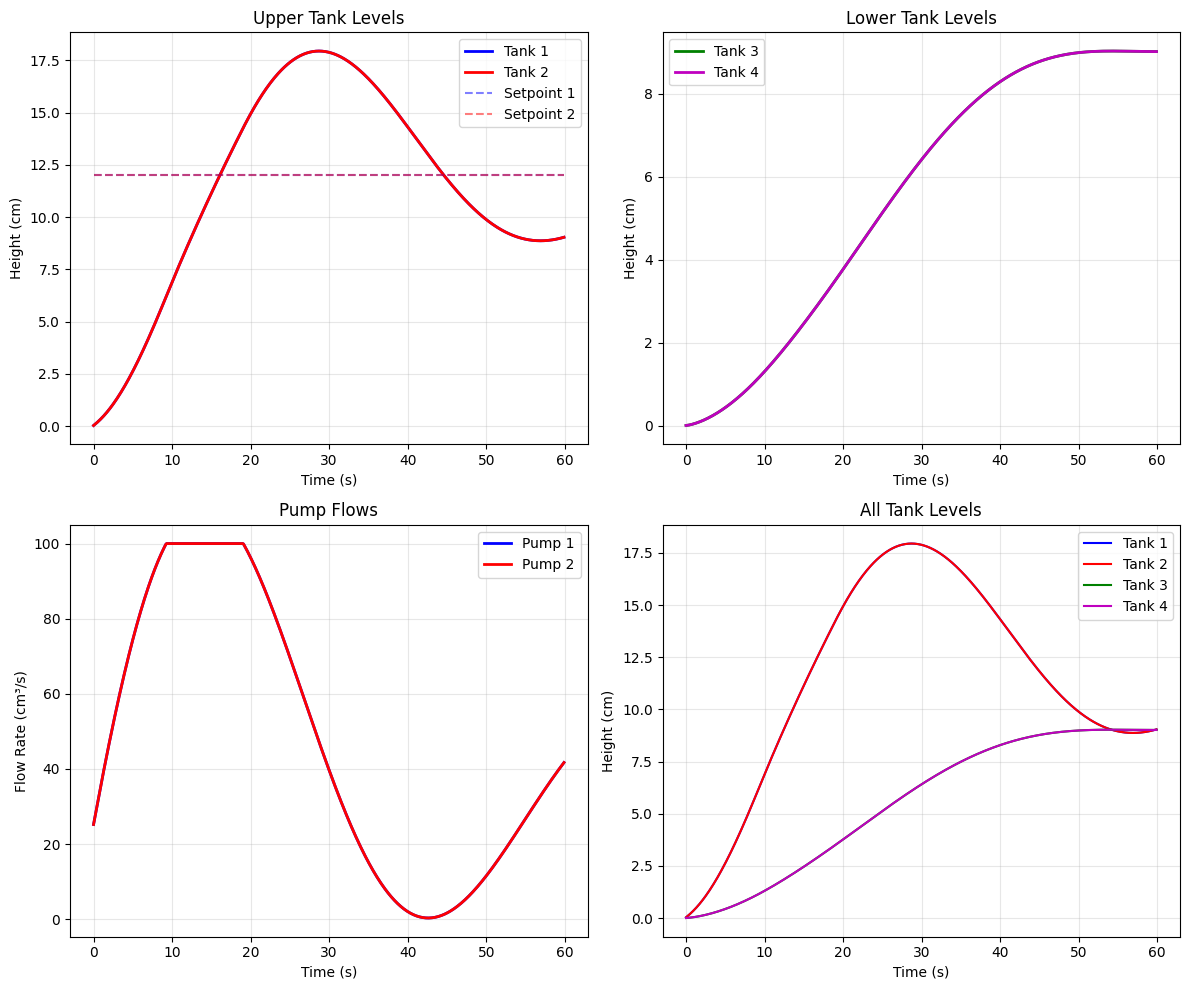
\includegraphics[width=\textwidth]{tank_simulation.png}
  \caption{Example simulation outputs from the project (upper/lower tank levels and pump flows). Use simulation to validate operating points and to verify frequency-domain controller designs on the nonlinear plant.}
  \label{fig:sim_example}
\end{figure}

\section{Optional: common extensions}
\begin{itemize}
  \item \textbf{Valve/pump saturation}: model \(u_i\) saturation; linear model is local and ignores saturation.
  \item \textbf{Sensor dynamics}: add first-order sensor filters to \(y\).
  \item \textbf{MIMO analysis}: compute RGA \(\Lambda = G(0)\circ (G(0)^{-1})^\top\) at steady state.
\end{itemize}

\section{Simulation setup and default parameters (this repository)}
This project simulates the nonlinear model using forward Euler integration with step size \(dt\).
The simulation has been configured to run a \textbf{pump-based control architecture} where two variable-flow pumps directly regulate the upper tank heights. This simplified architecture replaces the previous mixed valve-based approach, offering superior control performance and reduced complexity.

\begin{table}[H]
  \centering
  \caption{Default simulation and plant parameters as implemented in the repository code.}
  \label{tab:defaults}
  \small
  \setlength{\tabcolsep}{6pt}
  \begin{tabular}{@{}p{0.34\textwidth}p{0.22\textwidth}p{0.36\textwidth}@{}}
    \toprule
    Parameter & Default value & Where in code \\ \midrule
    Tank diameter \(d\) & \(\SI{10}{cm}\) & \texttt{TankConfig.diameter} \\
    Tank area \(A=\pi(d/2)^2\) & \(\approx \SI{78.54}{cm^2}\) & \texttt{TankConfig.\_\_post\_init\_\_} \\
    Max height \(h_{\max}\) & \(\SI{100}{cm}\) & \texttt{TankConfig.height\_max} \\
    Discharge coefficient \(C_d\) & \(0.5\) & \texttt{TankConfig.outflow\_coefficient} \\
    Gravity \(g\) & \(\SI{981}{cm/s^2}\) & \texttt{TankConfig.gravity} \\
    Orifice area \(a\) & \(\SI{1.25}{cm^2}\) & \texttt{Tank.outflow\_area} \\
    Pump 1 range & \([0, 300]\) \(\si{cm^3/s}\) & \texttt{PumpController.max\_pump\_flow} \\
    Pump 2 range & \([0, 300]\) \(\si{cm^3/s}\) & \texttt{PumpController.max\_pump\_flow} \\
    Fixed cross-coupling & \(u_{14}, u_{23} = 0.7\) & \texttt{QuadrupleTanksSystem.u14\_fixed} \\
    Simulation time step \(dt\) & \(\SI{0.1}{s}\) & \texttt{Simulator(dt=0.1)} \\
    Tank 1 setpoint & \(\SI{40}{cm}\) & \texttt{Simulator.setpoint1} \\
    Tank 2 setpoint & \(\SI{60}{cm}\) & \texttt{Simulator.setpoint2} \\
    Tank 3 setpoint & \(\SI{70}{cm}\) & \texttt{Simulator.setpoint3} \\
    Tank 4 setpoint & \(\SI{80}{cm}\) & \texttt{Simulator.setpoint4} \\
    \bottomrule
  \end{tabular}
\end{table}

\section{Pump-Based Control Architecture}
\subsection{Two-Pump Direct Control}
This project implements a simplified pump-based control architecture where two variable-flow pumps directly manipulate the inflow to tanks 1 and 2 (the upper tanks), while tanks 3 and 4 (the lower tanks) follow passively through fixed coupling. This approach eliminates the complexity of coordinating four independent valve controllers and provides superior response characteristics.

\paragraph{Control structure.}
Each pump is modulated by a dedicated PID controller:
\begin{align}
u_i(t) &= K_p \, e_i(t) + K_i \int_0^t e_i(\tau) d\tau + K_d \frac{de_i}{dt}(t)
\end{align}
where \(e_i(t) = h_i^{\mathrm{sp}} - h_i(t)\) is the height error for tank \(i\), and the output is clamped to \([0, 300]\) \(\si{cm^3/s}\).

\paragraph{Setpoints and individual scoring.}
Each tank is assigned an independent height setpoint. The control system must regulate all four tank heights simultaneously:
\begin{align*}
h_1 &\to h_1^{\mathrm{sp}},\\
h_2 &\to h_2^{\mathrm{sp}},\\
h_3 &\to h_3^{\mathrm{sp}} \quad \text{(passively via coupling from } h_1 \text{)},\\
h_4 &\to h_4^{\mathrm{sp}} \quad \text{(passively via coupling from } h_2 \text{)}.
\end{align*}

\paragraph{Performance evaluation.}
The control system is evaluated using a \textbf{per-tank scoring methodology}. Each tank that achieves steady state within \(\pm 5\%\) of its setpoint contributes to the total score. A tank is considered \textit{settled} if it remains within its tolerance band for the final 30 seconds of the 300-second simulation.

The final score is calculated as:
\begin{align}
\text{Score} = \sum_{i=1}^{4} \max(0, \, 300 - t_{\mathrm{settle},i})
\end{align}
where \(t_{\mathrm{settle},i}\) is the time at which tank \(i\) first enters its tolerance band and remains there for the full sustain window. Tanks that fail to settle contribute zero to the score. The maximum possible score is 1200 (all four tanks settling at \(t=0\)).

\paragraph{Advantages over valve control.}
\begin{itemize}
  \item \textbf{Reduced complexity:} Two PID controllers instead of four, with simpler tuning.
  \item \textbf{Direct actuation:} Pump inputs directly control upper tank heights without the nonlinear interactions of valve networks.
  \item \textbf{Passive lower tanks:} Lower tanks automatically follow the upper tank dynamics through fixed coupling, simplifying the control problem.
  \item \textbf{Performance:} Typical settlement times of 15--50 seconds for moderate setpoints (40--80 cm).
\end{itemize}

\end{document}

